\documentclass[main]{subfiles}

\begin{document}

\chapter{Manual de usuario del simulador}
\label{chap:anexo_simulador}

En este anexo se explica como utilizar el simulador implementado. 

\subsection*{Abriendo el programa}

\begin{enumerate}
\item Abrir el programa \emph{MatLab}.
\item Ubicarse en la carpeta uquad.
\item Desde la consola correr el script \emph{startup}. Este script agrega al \emph{path} las carpetas necesarias para que el simulador funcione adecuadamente.
\item Desde la consola correr el simulador ejecutando \emph{menu}. Un men\'u como el que se muestra en la figura \ref{fig:menu} deber\'ia aparecer.
\end{enumerate}

\begin{wrapfigure}{r}{0.6\textwidth}
\centering
  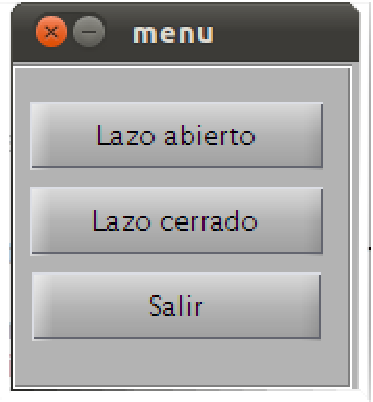
\includegraphics[width=0.2\textwidth]{./pics_anexo_simulador/menu.pdf}
\caption{Men\'u principal}
\label{fig:menu}
\end{wrapfigure}
Dicho men\'u ofrece la posibilidad de realizar simulaciones tanto en lazo abierto como en lazo cerrado haciendo ``click'' en la opci\'on deseada.\\

\subsection*{Simulaciones en lazo abierto}
Luego de hacer ``click'' en la opci\'on de lazo abierto en el men\'u principal se despliega el men\'u de la figura \ref{fig:anexo:lazo_abierto}. 

\subsubsection*{Estableciendo las condiciones iniciales de la simulaci\'on}
Para establecer las condiciones iniciales de la simulaci\'on se escribe el valor deseado para cada variable en el casillero correspondiente en la parte superior izquierda del men\'u. Las variables que se pueden establecer son:
\begin{itemize}
\item La posici\'on inicial del cuadric\'optero.
\item La orientaci\'on inicial (\'Angulos de Euler) del cuadric\'optero.
\item La velocidad inicial del cuadric\'optero en el sistema inercial.
\item La velocidad angular del cuadric\'optero.
\end{itemize}
\begin{figure}
\centering
  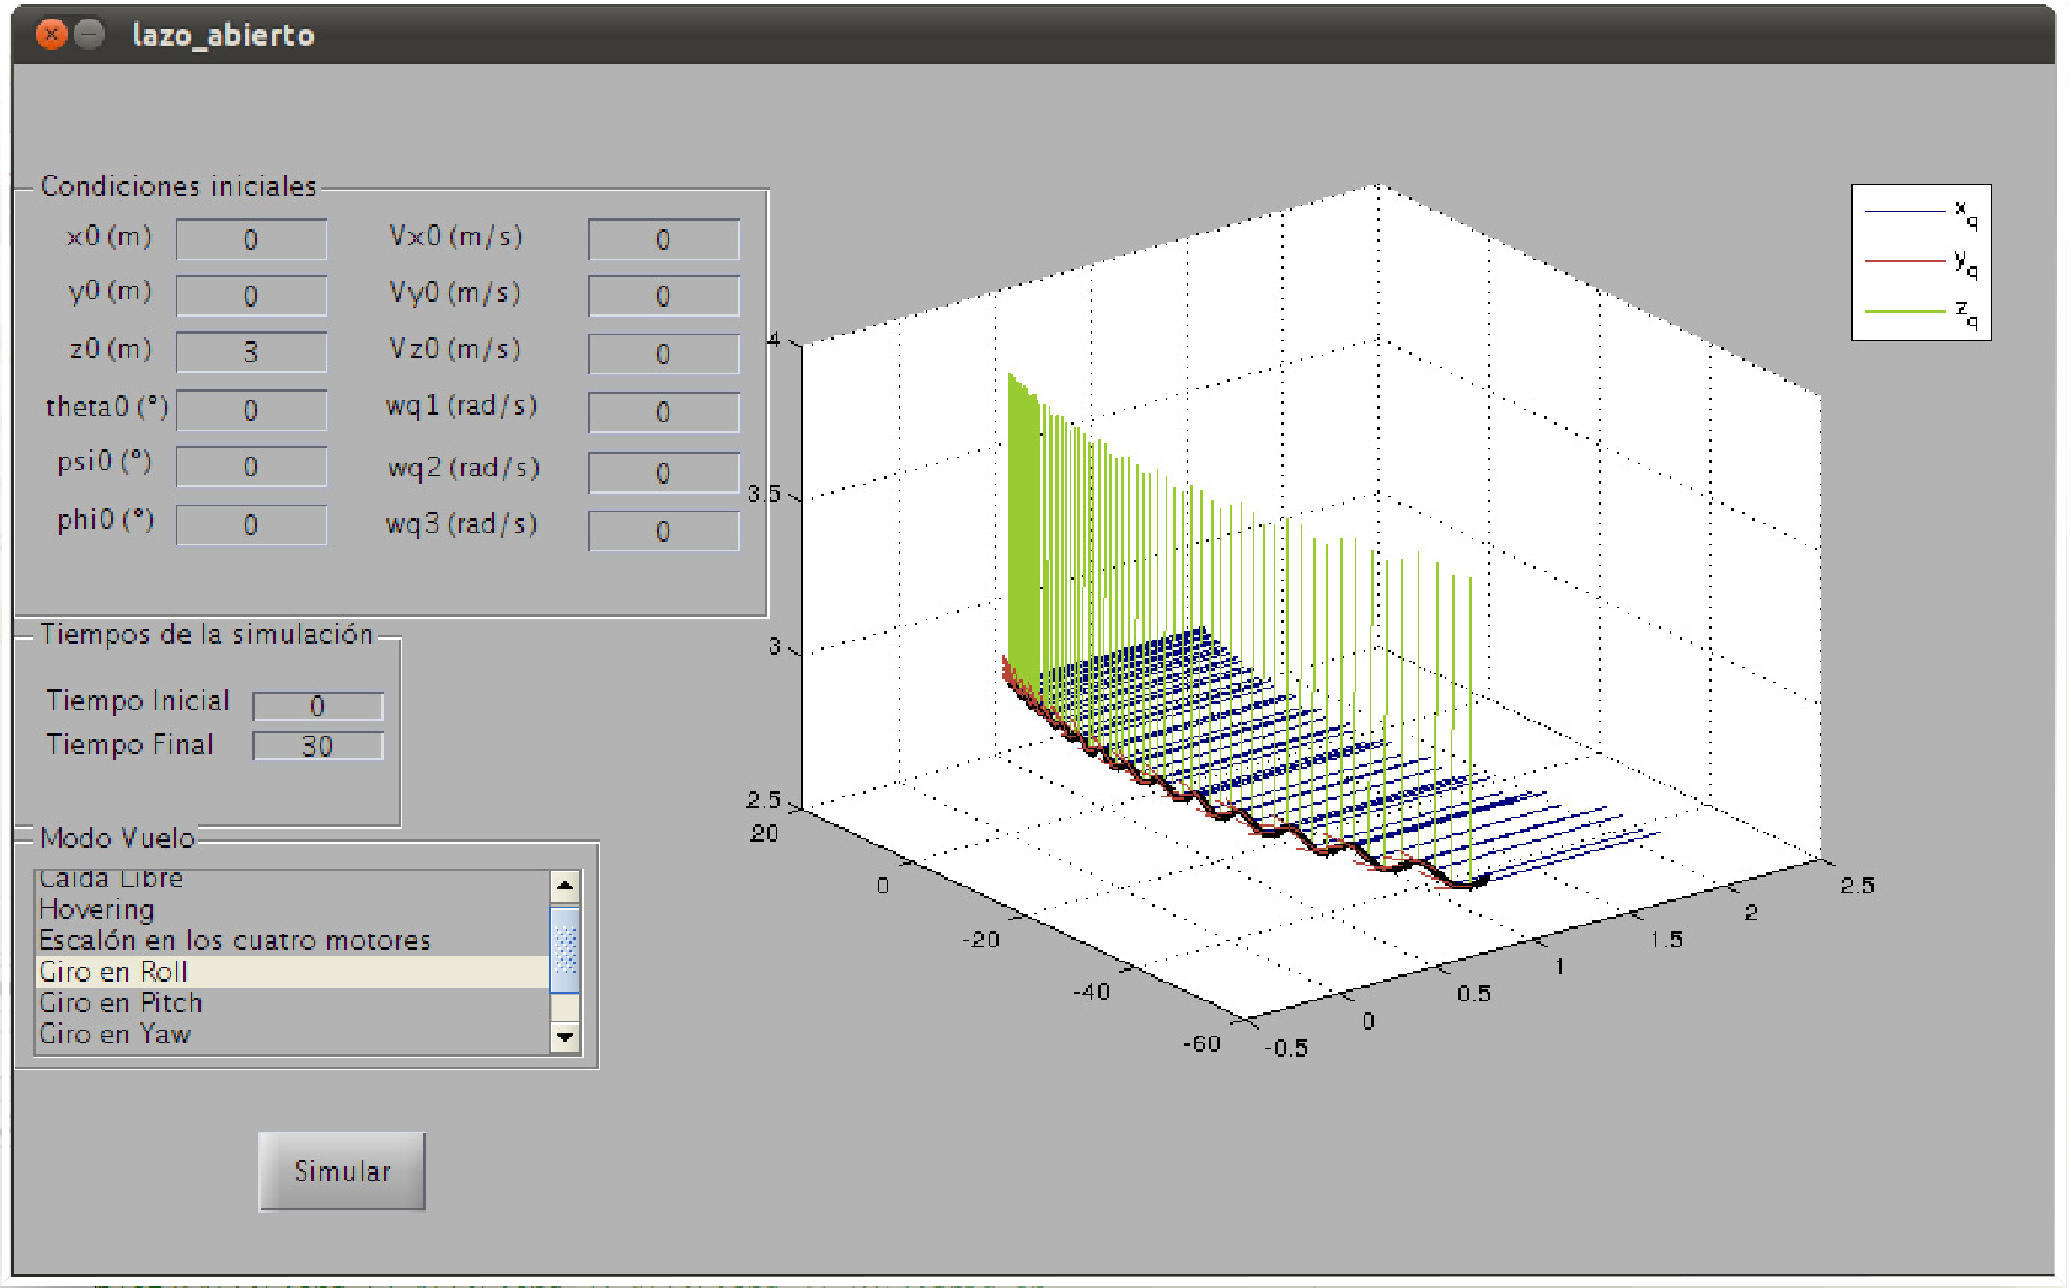
\includegraphics[width=0.8\textwidth]{./pics_anexo_simulador/anexo:lazo_abierto.pdf}
\caption{Interfaz del lazo abierto}
\vspace{-20pt}
\label{fig:anexo:lazo_abierto}
\end{figure}

En la figura \ref{fig:anexo:lazo_abierto} se realiz\'o una simulaci\'on con todas las condiciones iniciales nulas excepto la altura (z) que se fij\'o a tres metros.
\subsubsection*{Estableciendo los tiempos de la simulaci\'on}
La interfaz permite indicar los tiempos iniciales y finales de la simulaci\'on en el submen\'u que se encuentra al centro a la izquierda. En la figura se observa que para la simulaci\'on en cuesti\'on se estableci\'o un tiempo inicial de 0 segundos y un tiempo final de 30 segundos.

\subsubsection*{Estableciendo el modo de vuelo}
Con el submen\'u que se encuentra en la parte inferior se define el tipo de simulaci\'on que se desea realizar. El usuario puede elegir el modo de vuelo de una lista pre establecida, los modos de vuelo disponible son:
\begin{itemize}
\item Ca\'ida libre
\item Hovering
\item Escal\'on en los cuatro motores
\item Giro en Roll
\item Giro en Pitch
\item Giro en Yaw
\end{itemize}

\subsubsection*{Realizando la simulaci\'on}
Una vez establecidas las condiciones iniciales de la simulaci\'on, los tiempos iniciales y finales y el tipo de vuelo que se desea realizar se oprime el bot\'on simular para iniciar la simulaci\'on.\\

Sobre la derecha de la interfaz gr\'afica se despliega la trayectoria realizada por el sistema y la evoluci\'on de los ejes principales del cuadric\'optero: $x_q$, $y_q$ y $z_q$ en azul, rojo y verde respectivamente.\\

Para realizar un pos procesamiento de la informaci\'on obtenida gracias a la simulaci\'on es importante tener en cuenta que el simulador devuelve un vector con los tiempos de la simulaci\'on y una matriz con las 12 variables de estado. La variable de los tiempos de la simulaci\'on toma el nombre \textbf{t} y la variable con las 12 variabes de estado toma el nombre \textbf{Y}. Cada columna de la matriz \textbf{Y} representa los distintos valores que toma cada variable de estado a lo largo del tiempo. El \'orden en el cual se guardan las variables de estado es:
\begin{itemize}
\item Northing (x)
\item Westing (y)
\item Altura (z)
\item Roll ($\psi$)
\item Pitch ($\varphi$)
\item Yaw ($\vartheta$)
\item Velocidad en el sistema solidario al cuadric\'optero seg\'un $x_q$ ($v_{qx}$)
\item Velocidad en el sistema solidario al cuadric\'optero seg\'un $y_q$ ($v_{qy}$)
\item Velocidad en el sistema solidario al cuadric\'optero seg\'un $z_q$ ($v_{qz}$)
\item Velocidad angular del cuadric\'optero seg\'un $x_q$ ($\omega_{qx}$)
\item Velocidad angular del cuadric\'optero seg\'un $y_q$ ($\omega_{qy}$)
\item Velocidad angular del cuadric\'optero seg\'un $z_q$ ($\omega_{qz}$)
\end{itemize} 

\subsection*{Simulaciones en lazo cerrado}
Haciendo ``click'' en la opci\'on Lazo cerrado en el men\'u principal se despliega la interfaz que se muestra en la figura \ref{fig:anexo:lazo_cerrado}. Esta interfaz permite realizar simulaciones en lazo cerrado a fin de verificar el funcionamiento de los algoritmos de control.
\begin{figure}
\centering
  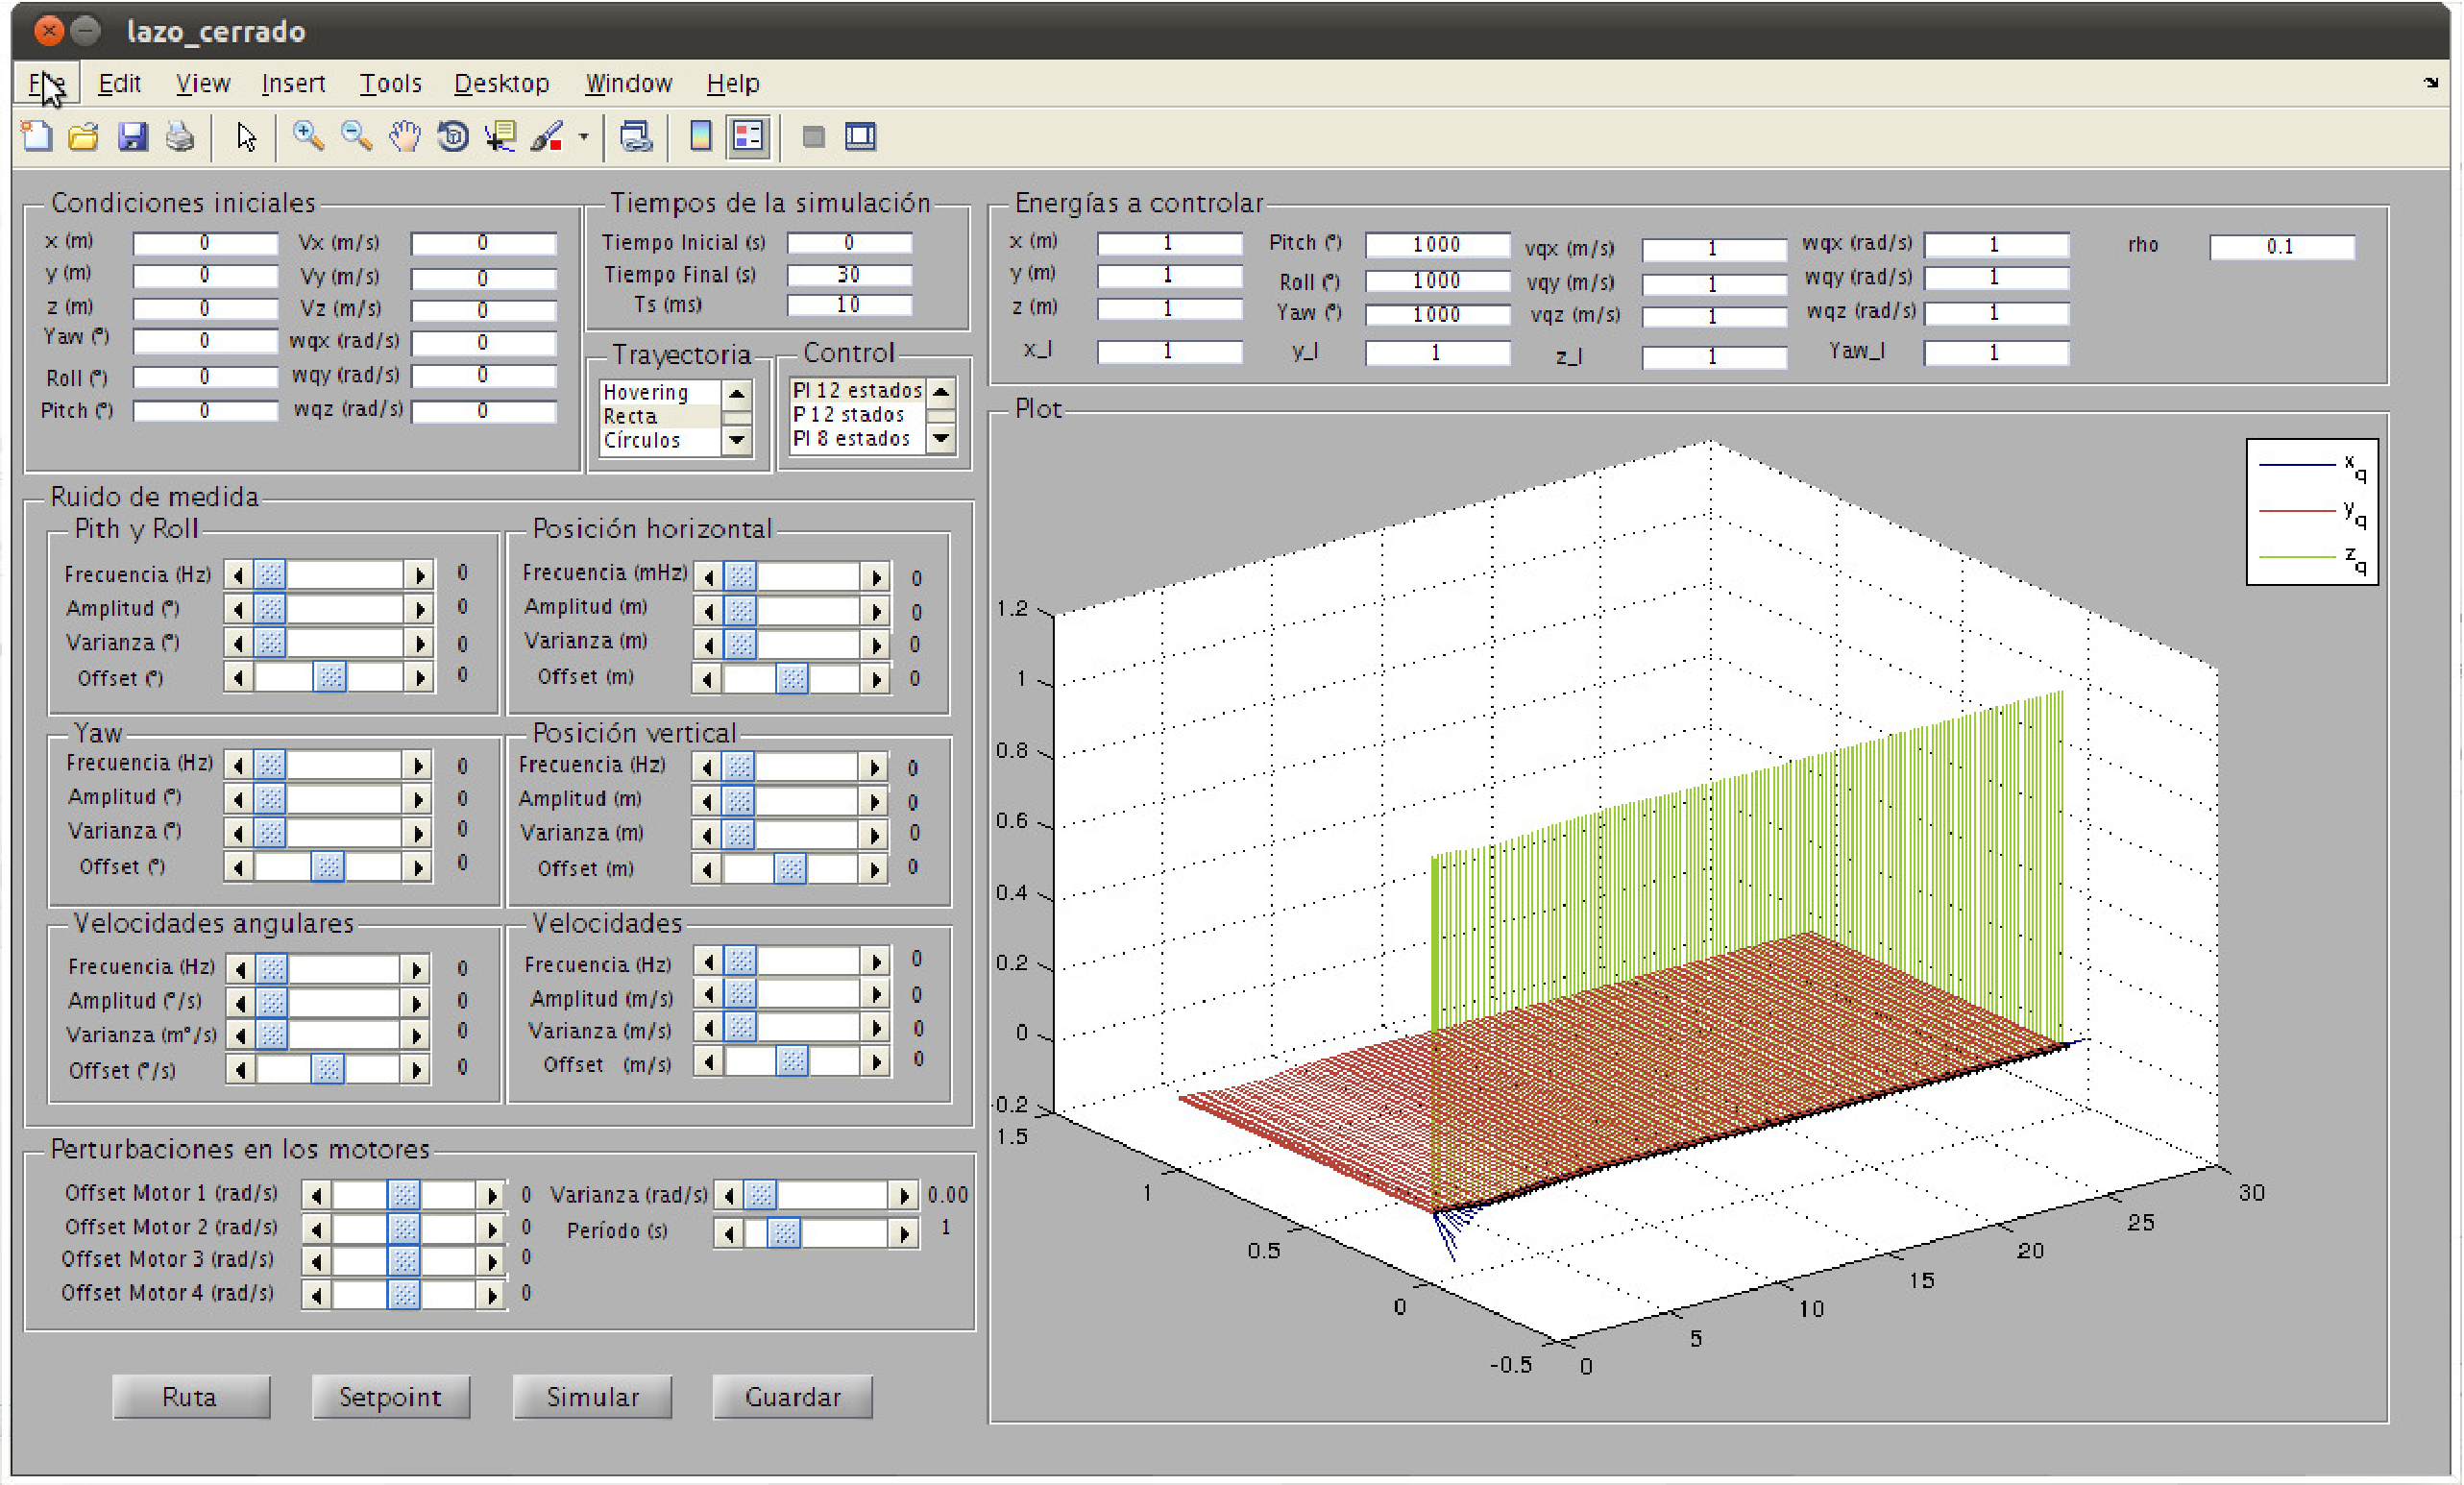
\includegraphics[width=0.8\textwidth]{./pics_anexo_simulador/anexo:lazo_cerrado.pdf}
\caption{Interfaz del lazo cerrado}
\vspace{-20pt}
\label{fig:anexo:lazo_cerrado}
\end{figure} 

\subsubsection*{Estableciendo las condiciones iniciales y tiempos de simulaci\'on}
En el submen\'u que se encuentra en la esquina superior izquierda de la interfaz pueden establecerse las condiciones iniciales de la simulaci\'on al igual que en la simulaci\'on en lazo abierto. A la derecha de dicho submen\'u se pueden establecer el tiempo inicial y final de la simulaci\'on al igual que en la simulaci\'on del lazo abierto.

\subsubsection*{Trayectoria a controlar}
En el panel Trayectoria puede elegirse el tipo de trayectoria a realizar. En esta versi\'on del simulador se tiene implementada tres trayectorias que pueden elegirse desde el men\'u:
\begin{itemize}
\item Hovering.
\item Vuelo en l\'inea recta.
\item Vuelo en c\'irculos.
\end{itemize}

Adem\'as del tipo de trayectoria deben establecerse los par\'ametros con los cuales se desea realizar la trayectoria. Para esto, haga ``click'' en el bot\'on \emph{setpoint} de la interfaz de lazo cerrado. Una nueva ventana se abrir\'a ofreciendo casilleros para completar con las variables deseadas. Seg\'un el tipo de trayectoria escogida se pueden setear distintas variables:
\begin{itemize}
\item Hovering: Posici\'on y \'angulo de Yaw.
\item Vuelo en l\'inea recta: Velocidades en el sistema $S_q$ y \'angulo de Yaw.
\item Vuelo en c\'irculos: Velocidad angular seg\'un la vertical y velocidad tangencial.
\end{itemize}

\subsection*{Controlador}
El simulador ofrece cuatro tipos de control posibles, seleccionables desde el panel \emph{Control} de la interfaz de lazo cerrado. Estos son:
\begin{itemize}
\item P12: controlador proporcional de todas las variables de estado del sistema.
\item PI12: controlador proporcional de todas las variables de estado del sistema y de las integrales del error en posici\'on y en el \'angulo de Yaw.
\item P8: controlador proporcional de ocho de las doce variables de estado del sistema. Se deja por fuera la posici\'on horizontal y las velocidades $v_{qx}$ y $v_{qy}$.
\item PI8: controlador id\'entico al anterior con el agregado del control sobre la integral del error en los tres \'angulos de euler y en la altura.
\end{itemize}

El control implementado es LQR. En el panel que se ubica en la esquina superior derecha se pueden variar los par\'ametros de las matrices Q y R utilizadas para determinar la matriz de realimentaci\'on. Se imponen dos restricciones para esta elecci\'on:
\begin{itemize}
\item Las matrices Q y R son diagonales
\item Todas las entradas de la matriz R son id\'enticas
\end{itemize}

\subsection*{Simulaci\'on}
Una vez establecidas las condiciones iniciales, los tiempos de la simulaci\'on, el tipo de trayectoria, el setpoint, el tipo de control y los par\'ametros de las matrices Q y R se puede proceder a simular el sistema en lazo cerrado haciendo ``click'' sobre el bot\'on simular.\\

En la gr\'afica de la derecha se grafica, al igual que para el lazo abierto, la trayectoria obtenida y los ejes del cuadric\'optero a lo largo del tiempo.\\

Se genera un vector \textbf{t} con los tiempos de la simulaci\'on y una matriz \textbf{Y} con la siguiente informaci\'on:
\begin{itemize}
\item En las primeras doce columnas de la matriz \textbf{Y} se guardan las variables de estado del sistema en el mismo \'orden que para el lazo abierto.
\item En las segundas doce columnas de la matriz \textbf{Y} se guardan los ruidos generados para las doce variables de estado en el mismo \'orden. (En las siguientes secciones se explica con mayor profundidad este aspecto).
\item Las columnas 25 a 28 de la matriz \textbf{Y} corresponden a las velocidades angulares de los cuatro motores a lo largo del tiempo.
\item Las columnas 29 a 40 corresponden al setpoint para cada variable de estado.
\end{itemize}

La matriz de realimentaci\'on generada puede ser guardada haciendo ``click'' sobre el bot\'on guardar. La matriz se guardar\'a en la carpeta \emph{./src/control/} bajo los siguientes nombres:
\begin{itemize}
\item PI12:
	\begin{itemize}
	\item K\_prop\_full.txt: matriz de realimentaci\'on proporcional.
	\item K\_int\_full.txt: matriz de realimentaci\'on para la integral del error de la posici\'on y el \'angulo de Yaw.
	\end{itemize}
\item P12: K\_full: matriz de realimentaci\'on proporcional.
\item PI8:
	\begin{itemize}
	\item K\_prop.txt: matriz de realimentaci\'on proporcional de ocho estados.
	\item K\_int.txt:  matriz de realimentaci\'on de la integral del error en los \'angulos de Euler y la altura.
	\end{itemize}
\item P8: K.txt: matriz de realimentaci\'on proporcional de ocho estados.
\end{itemize}

\subsection*{Ruido de medida y no idealidades}
El simulador ofrece la posibilidad de agregar ruido al estado que se utiliza para determinar la acci\'on de control. Este ruido simula los ruidos introducidos por los sensores. Para cada variable de estado puede agregarse desde el panel \emph{Ruido de medida} los siguientes ruidos:
\begin{itemize}
\item Componente sinusoidal. Puede ajustarse:
	\begin{itemize}
	\item Amplitud
	\item Frecuencia
	\end{itemize}
\item Ruido blanco: Puede ajustarse:
	\begin{itemize}
	\item Varianza
	\item Valor medio
	\end{itemize}
\end{itemize}

Puede agregarse tambi\'en en el panel \emph{Perturbaciones en los motores} offsets distintos para cada motor, y un ruido blanco (puede configurarse su varianza y per\'iodo) para simular el funcionamiento no ideal de los motores.\\

\subsubsection*{Ruta predeterminada}
El simulador ofrece adem\'as la posibilidad de recibir \emph{waypoints} por los cuales se desea pasar con una orientaci\'on determinada en un tiempo determinado. El simulador se encarga de concatenar las trayectorias a seguir para lograr el objetivo.\\

Todas las configuraciones descritas anteriormente son v\'alidas para esta secci\'on excepto que no tiene sentido definir una trayectoria ni los tiempos de simulaci\'on. Tampoco es posible guardar todas las matrices de realimentaci\'on utilizadas para lograr el objetivo planteado.\\

Para utilizar este modo:
\begin{enumerate}
\item Establecer las condiciones iniciales de la simulaci\'on, el controlador a utilizar, los ruidos y perturbaciones en los motores.
\item Hacer ``click'' sobre el bot\'on ruta. 
\item\label{enu:waypoint} En la ventana que se despliega establecer la posici\'on y la orientaci\'on del primer \emph{waypoint} as\'i como el tiempo en el cual se desea alcanzar dicho \emph{waypoint}.
\item\label{enu:waypoint_agregar} Hacer ``click'' sobre el bot\'on \emph{Agregar}.
\item Repetir los pasos \ref{enu:waypoint} y \ref{enu:waypoint_agregar} hasta agregar todos los puntos deseados.
\item Hacer ``click'' sobre el bot\'on \emph{Listo}.
\item Hacer ``click'' sobre el bot\'on \emph{Simular}.
\end{enumerate}

Al igual que para la simulaci\'on de una trayectoria en particular se guardan las variables \textbf{t} y \textbf{Y} para su posterior an\'alisis y estudio.

\end{document}

